\chapter{Gerenciamento do Projeto}
Neste capítulo, são abordadas as informações a respeito do gerenciamento do projeto, como a metodologia de gestão adotada, a organização da equipe, a gestão do tempo e as métricas levantadas ao longo do projeto.

\section{Metodologia de Gestão}
A metodologia de gerenciamento de projeto adotada é o \textit{Scrum}.

O \textit{Scrum} é um \textit{\gls{framework}} para gestão de projetos que tem como principais objetivos agilizar o processo de desenvolvimento de \textit{\gls{software}} e responder rapidamente às mudanças. Ela é composta por cerimônias e tem como um dos pilares as \textit{\glspl{sprint}}, ou seja, um conjunto de atividades para um determinado tempo. 

Essa metodologia foi adotada devido à experiência da maioria dos integrantes da equipe, que utilizam esse \textit{\gls{framework}} no ambiente de trabalho, e também por ser uma metodologia que demonstra ser eficaz para um gerenciamento de projetos.


No caso do projeto, as atividades de uma \textit{\gls{sprint}} são planejadas em uma \textit{Sprint Planning}, que é a primeira cerimônia e tem como principal objetivo a definição das entregas para o final da \textit{\gls{sprint}}. Nessa cerimônia, baseando-se nas histórias priorizadas no \textit{Product Backlog}, é criado o \textit{Sprint Backlog} em um arquivo em Excel, que contém as atividades e suas principais informações, como o responsável, o status, podendo ser \textit{To Do} (a fazer), \textit{Doing} (fazendo) e \textit{Done} (feito), e a data de conclusão. 


Após o planejamento da \textit{\gls{sprint}}, a execução das atividades é iniciada. A \textit{\gls{daily}} é feita através do aplicativo \textit{\gls{notion}}, no qual cada integrante coloca as atividades feitas no dia, os próximos passos e os impedimentos, caso houver. Além disso, reuniões de acompanhamento são feitas para ver o andamento do projeto e alinhamento das expectativas da \textit{\gls{sprint}}. Desse modo, esses \textit{\glspl{checkpoint}} semanais acontecem todas as terças-feiras às 19:30 ao longo da sprint. 

No último dia da \textit{\gls{sprint}}, às 19h30, é feita uma reunião para revisão das entregas, a chamada \textit{Sprint Review}, na qual é identificado o que foi entregue com sucesso, o que não foi concluído e também possíveis mudanças no \textit{\gls{product-backlog}}. 


Após a \textit{Sprint Review}, é feita uma reunião de retrospectiva, a \textit{Sprint Retrospective}, para avaliar o desempenho da equipe, o andamento do projeto e possíveis melhorias para a próxima \textit{\gls{sprint}}. E logo em seguida, a \textit{Sprint Planning} da \textit{\gls{sprint}} seguinte é realizada.


Todas as reuniões acontecem através do \textit{Google Meet}.
E para eventuais dúvidas, alinhamentos e possíveis urgências é utilizado o \textit{WhatsApp} e, caso houver necessidade, reuniões no \textit{Google Meet}. 


\section{Organização da Equipe}
As atividades foram divididas entre os integrantes da equipe segundo as habilidades e interesses de cada um, levando-se em consideração também o nível de dificuldade de cada frente.


Desse modo, o André é o \textit{\gls{tech-lead}} da equipe e foca na frente de desenvolvimento do sistema, portanto a parte de preparação do ambiente, desenvolvimento \textit{\gls{back-end}} e \textit{\gls{front-end}} são as suas principais atividades, mas também atuou na elaboração da documentação, na fase inicial do projeto, e como suporte, ao longo dele.

A Bianca é a gerente de projetos e \textit{\gls{scrum-master}} da equipe, sendo a responsável por garantir as entregas do projeto, por subir os arquivos no \ac{svn}, por ser a facilitadora em possíveis conflitos e impedimentos que possam surgir. Tem como principal foco a elaboração da documentação, além de ser responsável também pelas postagens semanais no blog.

O Luiz auxilia na elaboração da documentação, sendo, portanto, o seu principal foco, mas também auxiliou na frente de desenvolvimento do \textit{\gls{front-end}}, na elaboração de protótipos de alta e baixa fidelidade do sistema.

O Natan também compõe o time de desenvolvimento, auxiliando no desenvolvimento do \textit{\gls{back-end}} e do \textit{\gls{front-end}}. É o responsável pela criação, edição e postagem dos vídeos, mas também auxilia na elaboração da documentação, sobretudo na sua conversão para o LaTeX, e na subida dos arquivos no \ac{svn}.

A Patrícia é a \textit{\gls{product-owner}} da equipe, tendo como principal foco a documentação, lidando também com o \textit{\gls{product-backlog}} e elicitação de requisitos. Ela também auxilia na frente do desenvolvimento \textit{\gls{front-end}}, sobretudo na parte de protótipos de telas, testes e estilização das telas. 

Como uma das equipes da sala foi desfeita três semanas antes da entrega do \ac{mvp}, os integrantes que continuaram na disciplina foram alocados nas demais equipes. Foi nesse contexto que o Gustavo passou a integrar a equipe, fazendo parte do time de desenvolvimento e auxiliando tanto no desenvolvimento \textit{\gls{back-end}} quanto no \textit{\gls{front-end}}.

\section{Gestão de Tempo}

Baseando-se no Scrum, a gestão do tempo será feita pelas \textit{\glspl{sprint}}. Cada \textit{\gls{sprint}} terá a duração de duas semanas e, no total, serão quinze \textit{\glspl{sprint}}, com previsão de datas de início e de fim conforme descrito no \autoref{quadro-sprints}. 


\begin{quadro}[htb]
\centering
\ABNTEXfontereduzida
\caption{\label{quadro-sprints}Data de início e data fim de cada
\textit{sprint}}
\begin{tabular}{|c|c|c|}
   \hline
   \thead{Sprint} & \thead{Data Início}  & \thead{Data Fim}   \\\hline
    1 & 10/05/21 & 25/05/21 \\\hline
    2 & 25/05/21 & 08/06/21 \\\hline
    3 & 08/06/21 & 22/06/21 \\\hline
    4 & 22/06/21 & 06/07/21 \\\hline
    5 & 06/07/21 & 20/07/21 \\\hline
    6 & 20/07/21 & 03/08/21 \\\hline
    7 & 03/08/21 & 17/08/21 \\\hline
    8 & 17/08/21 & 31/08/21 \\\hline
    9 & 31/08/21 & 14/09/21 \\\hline
    10 & 14/09/21 & 28/09/21 \\\hline
    11 & 28/09/21 & 12/10/21 \\\hline
    12 & 12/10/21 & 26/10/21 \\\hline
    13 & 26/10/21 & 09/11/21 \\\hline
    14 & 09/11/21 & 23/11/21 \\\hline
    15 & 23/11/21 & 14/12/21 \\\hline
\end{tabular}
\fonte{Os autores}
\end{quadro}
\FloatBarrier


As atividades priorizadas para cada \textit{\gls{sprint}} foram baseadas no cronograma da disciplina e podem ser visualizadas no \autoref{sprints-atividades}.


\section{Métricas}
Uma vez por mês, foram levantados métricas a respeito do andamento do projeto. O \autoref{quadro-metricas} representa os resultados obtidos.
\begin{quadro}[htb]
\centering
\ABNTEXfontereduzida
\caption{\label{quadro-metricas}Métricas Gerais}
\begin{tabular}{|c|c|c|c|}
   \hline
   \thead{Métricas} & \thead{Maio} \footnote[ 1]{Começo em 10 de maio} & \thead{Junho}  & \thead{Julho}\footnote[ 2]{Medido até dia 18 de julho}   \\\hline
    Reuniões & 5 & 5 & 2 \\\hline
    Vídeos & 1 & 2 & 1 \\\hline
    Postagens no blog & 3 & 4 & 3 \\\hline
    Arquivos na pasta do SVN & 11 & 99 & 119 \\\hline
    Commits & 3 & 25 & 56 \\\hline
    Entidades no back-end & 1 & 2 & 11 \\\hline
    Linhas de código & 13 & 15859 & 25347 \\\hline
\end{tabular}
\fonte{Os autores}
\end{quadro}
\FloatBarrier

\subsection{Relatórios StatSVN}
A ferramenta \textit{StatSVN} foi utilizada para extrair relatórios a respeito do histórico do repositório da equipe no \gls{svn} e assim pôde-se obter dados estatísticos a respeito do desenvolvimento do projeto.

As Figuras \ref{fig:activity} e \ref{fig:commitsauthors} demonstram, respectivamente, as atividades dos integrantes da equipe e os \textit{commits} realizados por eles. Com esses gráficos, torna-se evidente que apenas dois integrantes atualizaram o repositório. Isso aconteceu porque o principal repositório usado para o versionamento de código foi o \textit{GitHub}, mas como o \gls{svn} é um dos requisitos para a disciplina, dois integrantes ficaram responsáveis por atualizar o repositório.
\begin{figure}[htb]
    \centering
	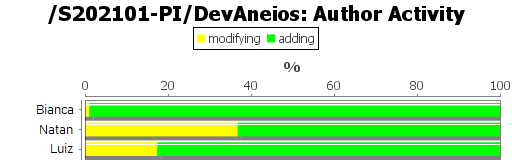
\includegraphics[width=16cm]{imagens/activity.png}
	\caption{\label{fig:activity} Atividades dos integrantes}
	\fonte{Os autores}
\end{figure}
\FloatBarrier

\begin{figure}[htb]
    \centering
	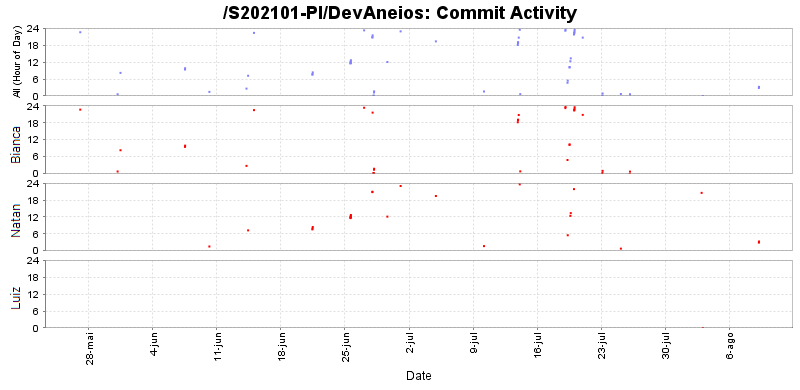
\includegraphics[width=16cm]{imagens/commitscatterauthors.png}
	\caption{\label{fig:commitsauthors} Commits por autor}
	\fonte{Os autores}
\end{figure}
\FloatBarrier

A \autoref{fig:day} demonstra os \textit{commits} da equipe por dia da semana. Com esse gráfico, é possível notar que os dias que mais foram realizados \textit{commits} foram na terça-feira e segunda-feita, que representam os dias que acontecem os \textit{checkpoints} semanais da equipe e as entregas da disciplina, respectivamente.

\begin{figure}[htb]
    \centering
	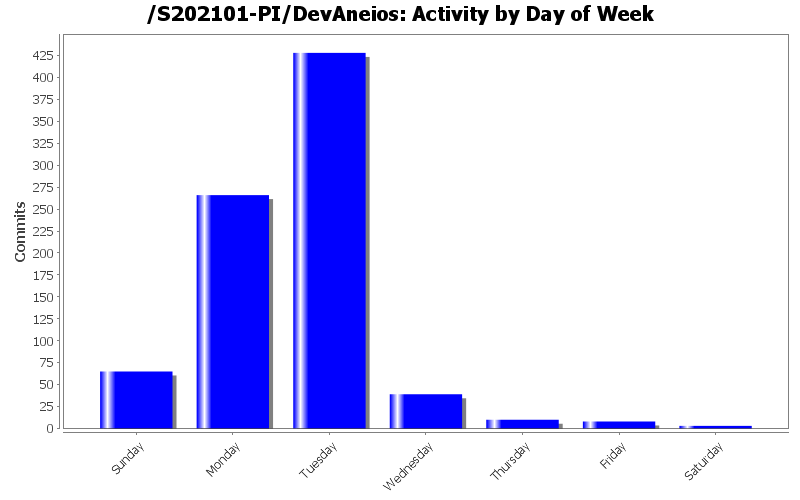
\includegraphics[width=16cm]{imagens/activity_day.png}
	\caption{\label{fig:day} Atividades por dia na semana}
	\fonte{Os autores}
\end{figure}
\FloatBarrier

A \autoref{fig:time} demonstra os \textit{commits} da equipe por horas do dia. Com esse gráfico, é possível verificar que os horários que mais foram feitos \textit{commits} foram de madrugada e na hora do almoço, representado os horários do dia que os integrantes tinham mais disponibilidade para se dedicar ao projeto.

\begin{figure}[htb]
    \centering
	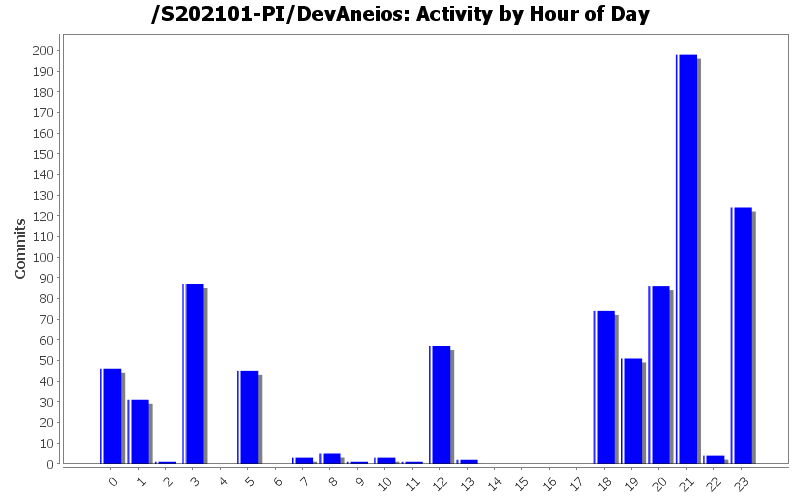
\includegraphics[width=16cm]{imagens/activity_time.png}
	\caption{\label{fig:time} Atividades por hora no dia}
	\fonte{Os autores}
\end{figure}
\FloatBarrier

A \autoref{fig:loc} demonstra a quantidade de linhas de código pelos dias ao longo dos meses. Com esse gráfico, é possível observar uma pequena curva de crescimento no início do projeto e um crescimento acentuado no dia 28 de junho, isso aconteceu pois na fase inicial do projeto, subiram-se apenas as documentações e, a partir do dia 28 de junho, passou-se a atualizar o \gls{svn} com o desenvolvimento do projeto.

\begin{figure}[htb]
    \centering
	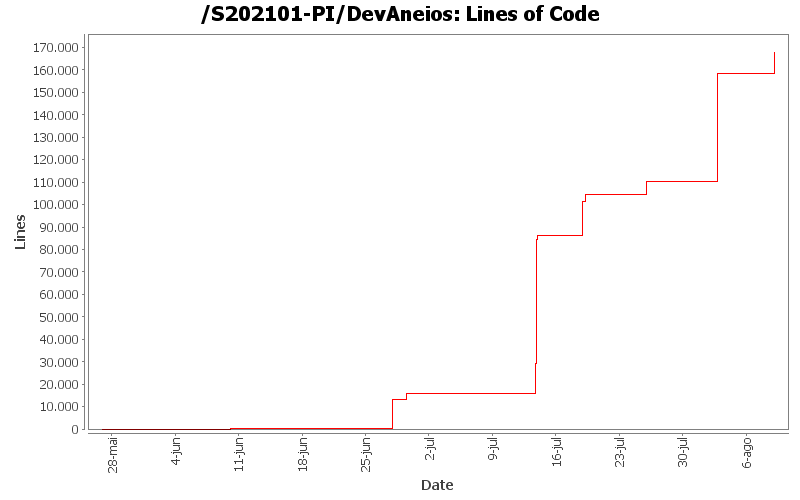
\includegraphics[width=16cm]{imagens/loc.png}
	\caption{\label{fig:loc} Linhas de código}
	\fonte{Os autores}
\end{figure}
\FloatBarrier

\section{Links de acesso}

Os \textit{\glspl{link}} de acesso pertinentes ao projeto estão disponíveis nesta seção.

A \autoref{qr-github} contém o \textit{\gls{qr-code}} que leva ao principal repositório remoto utilizado para o versionamento de código durante o desenvolvimento da aplicação, o \textit{GitHub}.
A fim de obter uma melhor divisão lógica, foram criados dois repositórios na plataforma para hospedar os códigos relacionados ao \textit{\gls{front-end}} e ao \textit{\gls{back-end}} do projeto.

\begin{figure}[htb]
\begin{flushright}
\begin{pspicture}(25mm,25mm)
\psbarcode{https://github.com/devaneios-ifsp}{eclevel=H width=1.0 height=1.0}{qrcode}
\end{pspicture}
\caption{\label{qr-github}\textit{QR-Code} - Repositório remoto GitHub}
\legend{\url{https://github.com/devaneios-ifsp}}
\fonte{Os Autores}
\end{flushright}
\end{figure}
\FloatBarrier


Além do GitHub, o repositório Subversion também foi utilizado para gerenciamento do código produzido, sendo atualizado periodicamente. A \autoref{qr-svn} contém o \textit{\gls{qr-code}} do repositório em questão.

\begin{figure}[htb]
%\begin{flushright}
\begin{pspicture}(25mm,25mm)
\psbarcode{https://svn.spo.ifsp.edu.br/viewvc/A6PGP/S202101-PI/DevAneios/}{eclevel=H width=1.0 height=1.0}{qrcode}
\end{pspicture}
\caption{\label{qr-svn}\textit{QR-Code} - Repositório remoto Subversion}
\legend{\url{https://svn.spo.ifsp.edu.br/viewvc/A6PGP/S202101-PI/DevAneios/}}
\fonte{Os Autores}
%\end{flushright}
\end{figure}
\FloatBarrier

Todos os vídeos produzidos pela equipe podem ser acessados no canal do Youtube da mesma, cujo \gls{link} está contido no \textit{\gls{qr-code}} da \autoref{qr-yt}.

\begin{figure}[htb]
\begin{flushright}
\begin{pspicture}(25mm,25mm)
\psbarcode{https://www.youtube.com/channel/UCjwYXnZHuCg74AkhR5aZs6A/featured}{eclevel=H width=1.0 height=1.0}{qrcode}
\end{pspicture}
\caption{\label{qr-yt}\textit{QR-Code} - Canal DevAneios no Youtube}
\legend{\url{https://www.youtube.com/channel/UCjwYXnZHuCg74AkhR5aZs6A/featured}}
\fonte{Os Autores}
\end{flushright}
\end{figure}
\FloatBarrier

Os relatórios semanais de atividades realizadas por cada membro do projeto são publicadas no blog da equipe, cujo \gls{link} pode ser acessado no \textit{\gls{qr-code}} da \autoref{qr-blog}.

\begin{figure}[htb]
%\begin{flushright}
\begin{pspicture}(25mm,25mm)
\psbarcode{https://devaneiosifsp.blogspot.com/}{eclevel=H width=1.0 height=1.0}{qrcode}
\end{pspicture}
\caption{\label{qr-blog}\textit{QR-Code} - Blog DevAneios}
\legend{\url{https://devaneiosifsp.blogspot.com/}}
\fonte{Os Autores}
%\end{flushright}
\end{figure}
\FloatBarrier

A página de login e cadastramento do site Turma de Elite pode ser acessada através do {\gls{qr-code}} na \autoref{qr-login}, com as credenciais informadas.

\begin{figure}[htb]
\begin{flushright}
\begin{pspicture}(25mm,25mm)
\psbarcode{https://turma-de-elite-app.web.app/login}{eclevel=H width=1.0 height=1.0}{qrcode}
\end{pspicture}
\caption{\label{qr-login}\textit{QR-Code} - Tela de Login Turma de Elite}
\legend{\url{https://turma-de-elite-app.web.app/login}}
\fonte{Os Autores}
\end{flushright}
\end{figure}
\FloatBarrier

Para acessar a aplicação, usar o seguinte e-mail e senha:
\begin{itemize}
    \item E-mail: admteste6@gmail.com
    \item Senha: 123456
\end{itemize}

Os detalhes da API do projeto são documentados na aplicação Swagger. Seu \gls{link} de acesso pode ser encontrado através do {\gls{qr-code}} da \autoref{qr-swagger}.

\begin{figure}[htb]
%\begin{flushright}
\begin{pspicture}(25mm,25mm)
\psbarcode{https://turma-de-elite.herokuapp.com/swagger-ui/}{eclevel=H width=1.0 height=1.0}{qrcode}
\end{pspicture}
\caption{\label{qr-swagger}\textit{QR-Code} - Swagger do Turma de Elite}
\legend{\url{https://turma-de-elite.herokuapp.com/swagger-ui/}}
\fonte{Os Autores}
%\end{flushright}
\end{figure}
\FloatBarrier
